\part{Profilers}
\frame{\partpage}

\begin{frame}{Unity Profiler}
	\begin{itemize}
		\pause \item The Unity Profiler is built into the engine
		\pause \item It can be accessed via the \textbf{ Window > Profiler}
		\pause \item This allows you to profile the following
		\begin{itemize}
			\pause \item CPU Usage - Scripts, Physics, UI etc
			\pause \item Rendering - Batches, Triangles, Vertices
			\pause \item Memory - Total, Texture, Mesh, Garbage Collection
			\pause \item Audio - Number of Sources, Audio Memory
			\pause \item GPU - Deferred Lighting, Transparent, Post Processing
		\end{itemize} 
	\end{itemize}
\end{frame}

\begin{frame}{Unity Profiler}
	\begin{figure}
		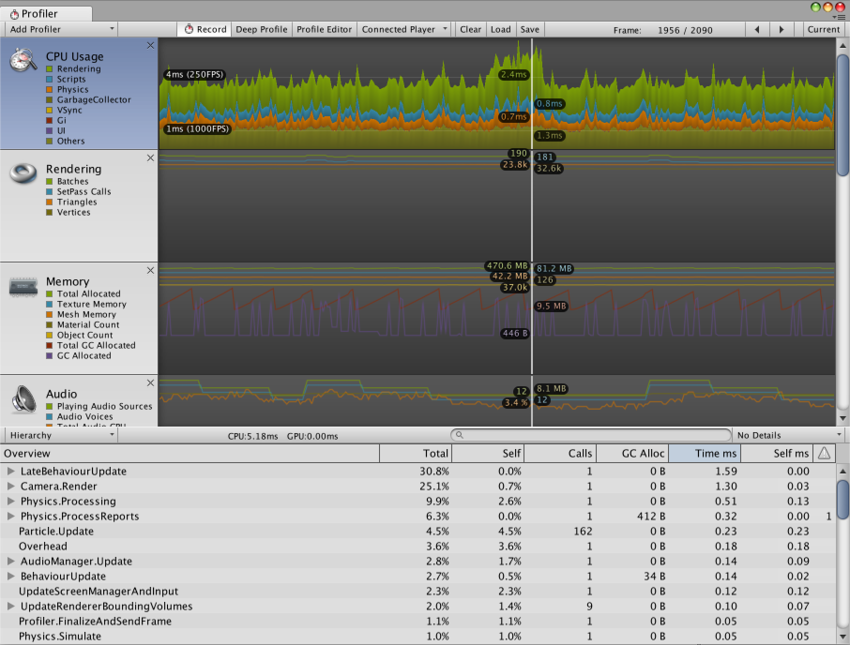
\includegraphics[width=1.0\textwidth,height=0.8\textheight]{UnityProfilerWindow}  
	\end{figure}
\end{frame}

\begin{frame}{Unity Profiler: Hints \& Tips}
	\begin{itemize}
		\pause \item You can remove items from the profiler graph by click on the colour box
		\pause \item Enabling \textbf{Deep Profile} will add a significant overhead to larger games
		\begin{itemize}
			\pause \item Surround you code with \textbf{Profiler.BeginSample} \& \textbf{Profiler.EndSample} this will appear in the Profiler
		\end{itemize}
		\pause \item You should consider Profiling a development build as the Editor adds significant overheard
	\end{itemize}
\end{frame}

\begin{frame}{Unreal Profiler}
	\begin{itemize}
		\pause \item The Unreal Profiler is built into the engine
		\pause \item It can accessed via \textbf{Window > Developer Tools > Session Frontend}
		\pause \item Allows us to profile all major systems including CPU (code) and GPU
	\end{itemize}
\end{frame}

\begin{frame}{Unreal Profiler}
	\begin{figure}
		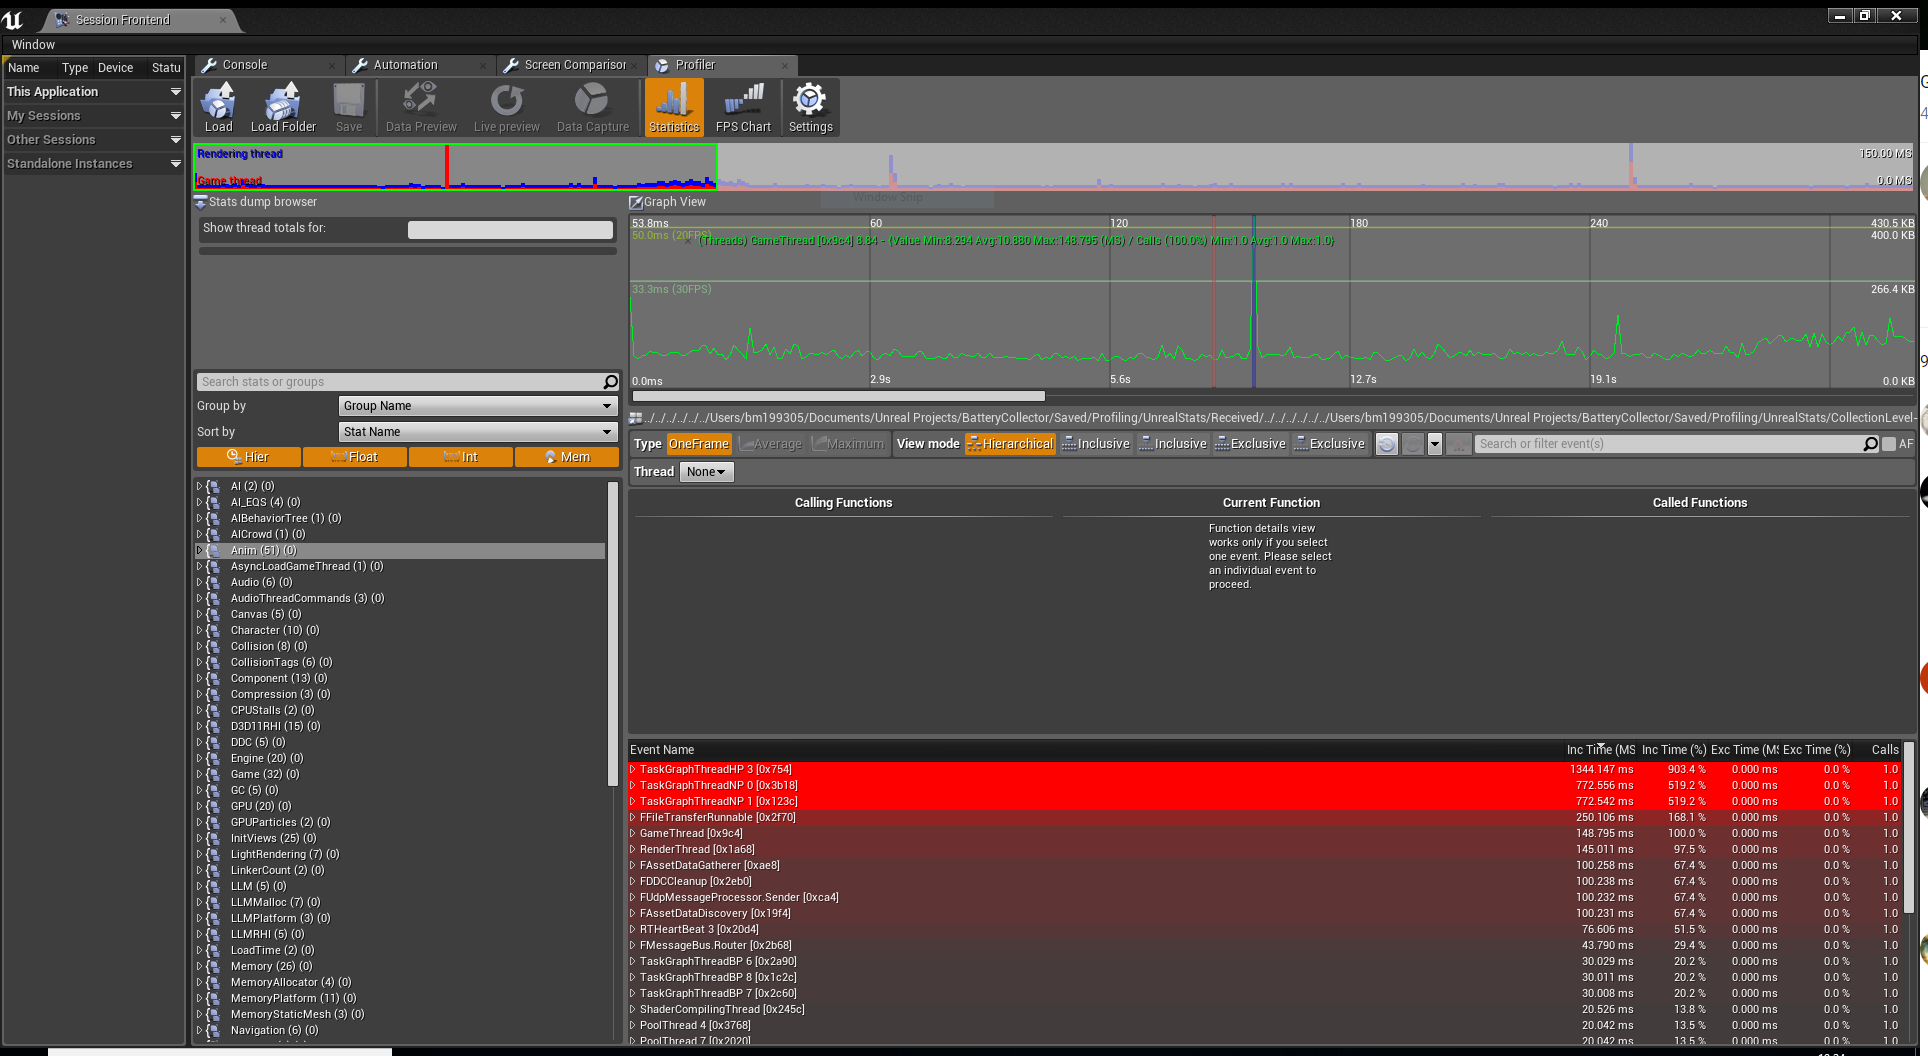
\includegraphics[width=1.0\textwidth,height=0.8\textheight]{UnrealProfilerWindow}  
	\end{figure}
\end{frame}

\begin{frame}{Unreal Profiler: Hints \& Tips}
\begin{itemize}
	\pause \item \url{https://www.unrealengine.com/en-US/blog/how-to-improve-game-thread-cpu-performance}
	\pause \item A few interesting things from this link
	\begin{itemize}
		\pause \item To identify the bottleneck (GPU or CPU), run \textbf{stat unit} on a \textbf{non-debug build}
		\pause \item If the \textbf{Frame Time} is very close to \textbf{GPU Time}, then the GPU is the bottleneck
		\pause \item If the \textbf{Frame Time} is very close to \textbf{Game Time}, then your code is the bottleneck
		\pause \item In the profiler \textbf{GameThread} entry, find the \textbf{FTickFunctionTask} - this shows every actor and component that is ticking
		\pause \item Another thing to track is \textbf{Blueprint Time}, switch inclusive view and locate it, then switch back to hierarchical view
		\pause \item \textbf{SkinnedMeshComp Tick} \& \textbf{TickWidgets} can also be bottleneck
	\end{itemize}
\end{itemize}
\end{frame}

\begin{frame}{ Visual Studio Profiler}
\begin{itemize}
	\pause \item \url{https://msdn.microsoft.com/en-us/library/ms182372.aspx}
	\pause \item Switch your application to a release build
	\pause \item To run the profiler, select \textbf{Debug > Performance Profiler} and then click on \textbf{Performance Wizard}
	\pause \item The profiler will run and start collecting data
	\pause \item Close the application to start analysing the data
\end{itemize}
\end{frame}


\begin{frame}{Visual Studio Profiler}
\begin{figure}
	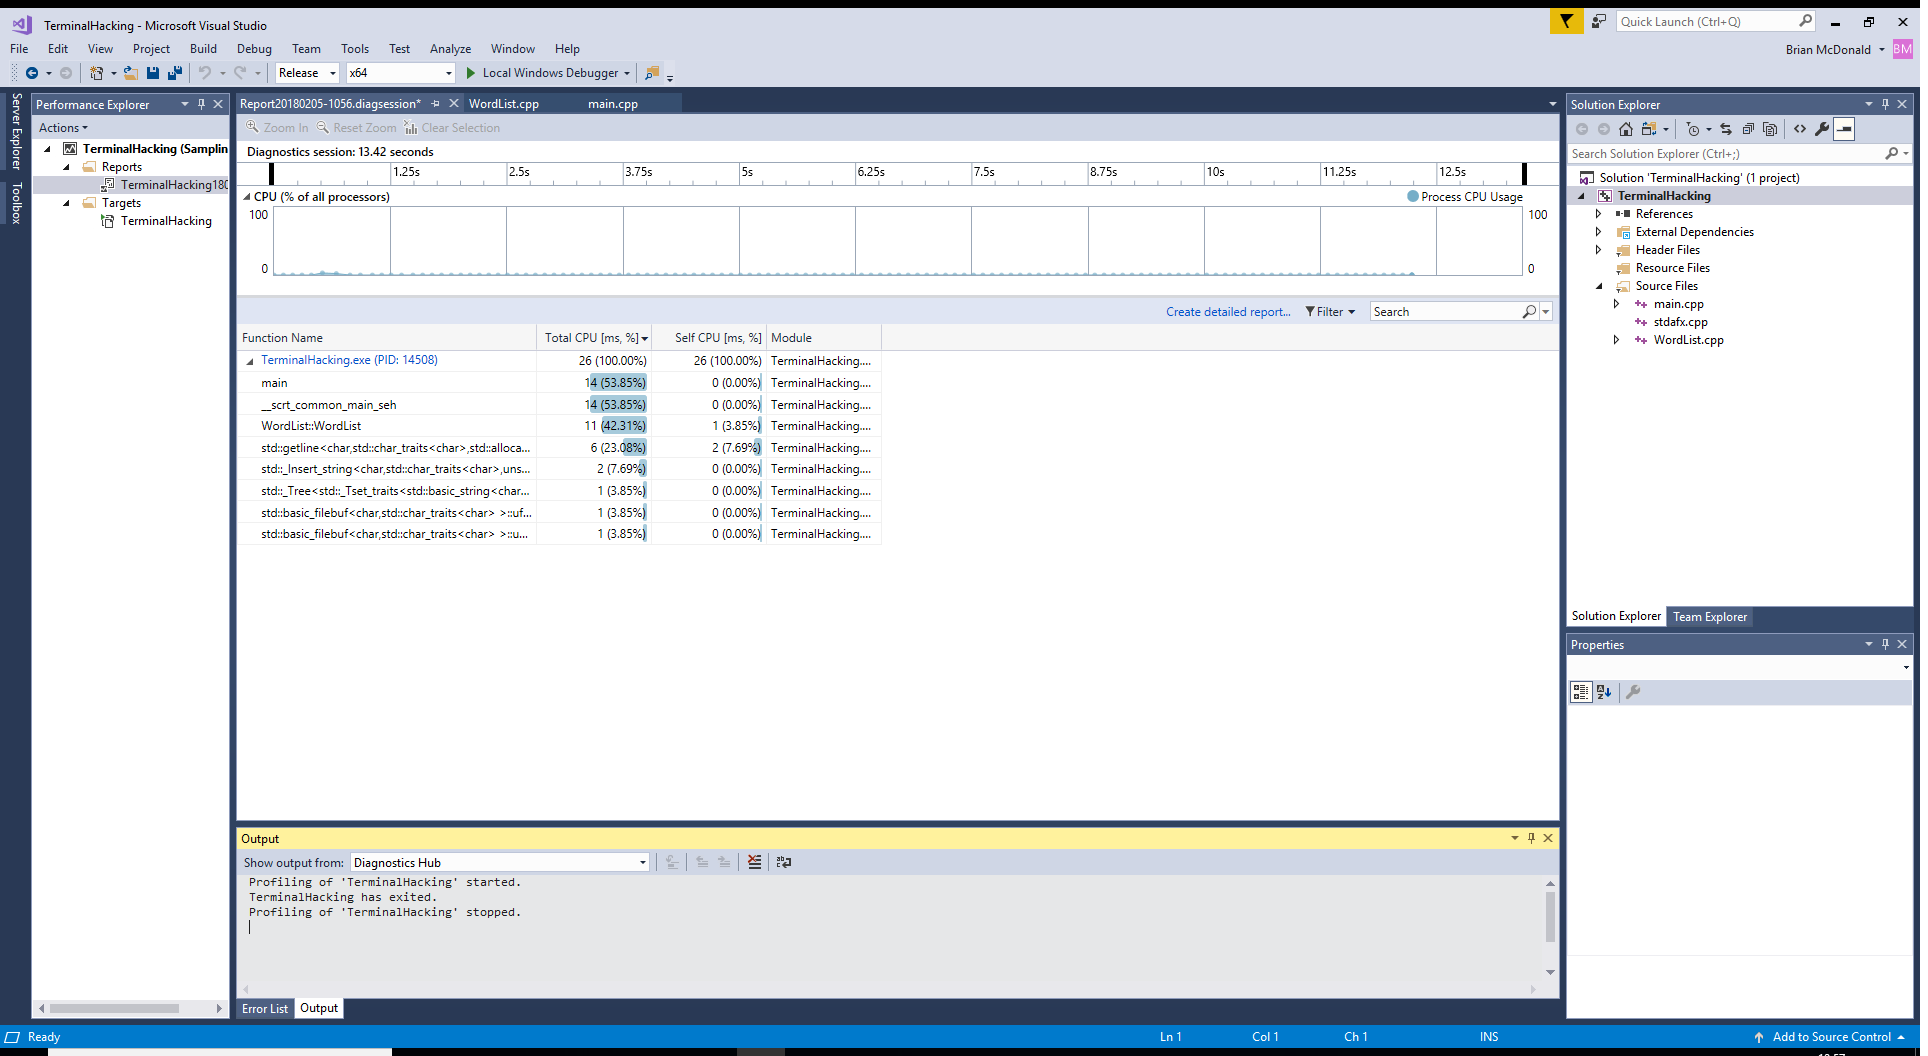
\includegraphics[width=1.0\textwidth,height=0.8\textheight]{VSProfilerWindow}
\end{figure}
\end{frame}

\begin{frame}{Visual Studio: Hints \& Tips}
\begin{itemize}
	\pause \item Click on \textbf{Create Detailed Report} in the summary view, this will generate a report on your application
	\pause \item In this report \textbf{Show Hot Lines} will show the code paths which do the  most work
	\pause \item You will not be able to do much about the *.dll calls, you should look at your own functions in here
\end{itemize}
\end{frame}
